\newpage
\section{Aufbau}
\label{sec:Aufbau}
Der hier untersuchte Si-Streifendetektor (EASy) der Firma Alibava setzt sich aus einer Kontroll- und einer Detektoreinheit, sowie ein Computer mit Steuer-Software zusammen. Eine ausführliche Beschreibung zur Funktionsweise und den Möglichkeiten des EASy-Systems lässt sich in der Anleitung von Alibava finden \cite{alibava}.

\subsection{Detektoreinheit}
\label{sec:Detektoreinheit}
 Die Detektoreinheit besteht aus einem Si-Streifenhalbleitersensor und der zugehörigen Ausleseelektronik. Der Sensor hat eine Gesamtdicke von \SI{300}{\micro\meter} und besteht aus 128 einzelnen p-dotierten Streifen in dem n-dotierten Siliziumbulk. Die Unterseite bildet eine Metallisierung, die zum Anschließen der Depletionsspannung dient. Oberhalb dieser Streifen befinden sich kapazitiv gekoppelte Elektroden aus Aluminium, die an den Pads mit Wirebonds an die Ausleseelektronik angeschlossen sind. Um ein direktes Abfließen des Leckstroms in diese zu verhindern, sind beide Komponenten durch eine Siliziumoxid-Schicht getrennt. Denn ein solches direktes Abfließen könnte die empfindliche Elektronik zerstören. Um ein unkontrolliertes Abfließen von Oberflächenströme zu verhindern, sind zudem Guard-Ringe um das Streifensystem gelegt. Um die Streifen mit einer Spannung versorgen zu können, sind die p-Implantate mit einem Ohmschen Widerstand an den Bias-Ring angeschlossen.
 Ein schematisches Darstellung des Sensors ist in Abbildung \ref{fig:schema} zu erkennen.
 \begin{figure}[htb]
   \centering
   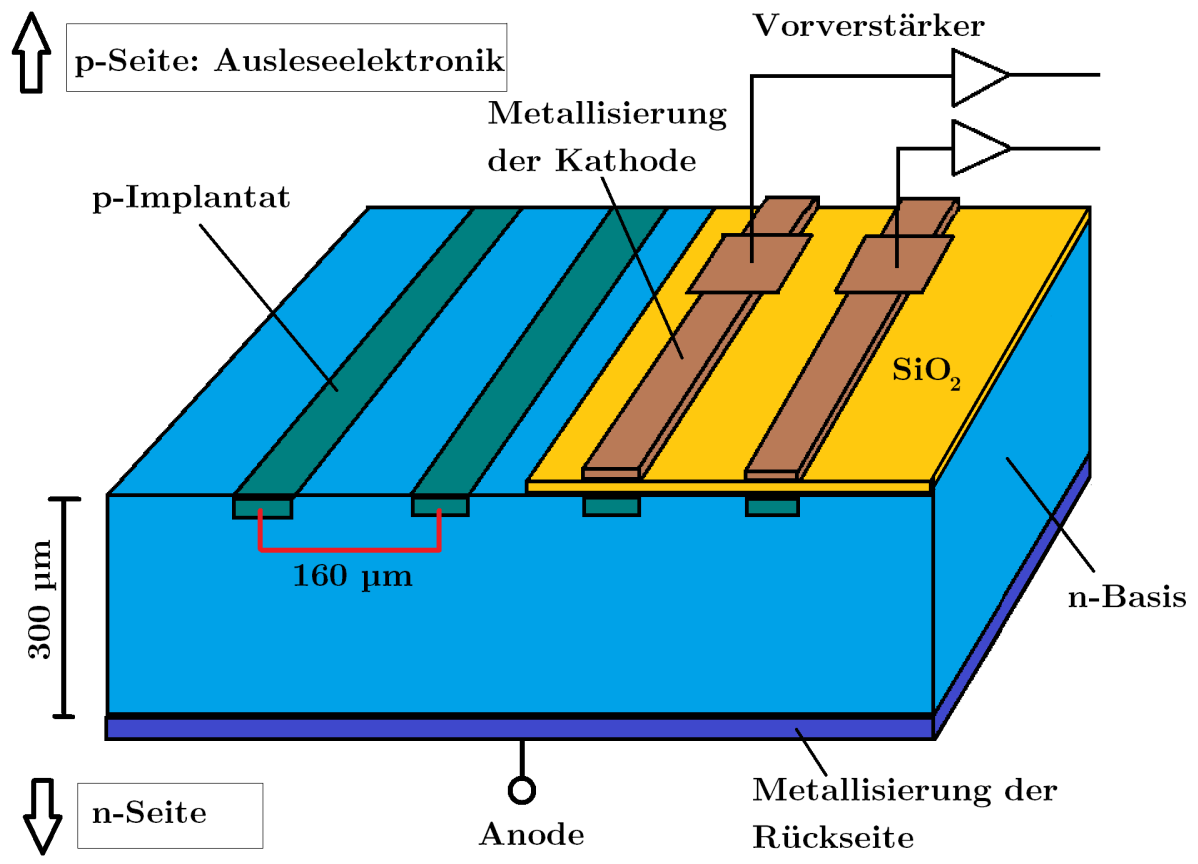
\includegraphics[width=0.7\textwidth]{graphics/Schema.png}
   \caption{Schematische Darstellung eines Si-Streifensensors mit Spannungsanschluss \cite{anleitung}.}
   \label{fig:schema}
 \end{figure}
Die makroskopische Aufnahme in Abbildung \ref{fig:streifendetektor} ermöglicht einen Überblick über die Position der Pads, den Widerständen, des Bias-Ring und den Guard-Ringen.
\begin{figure}[htb]
  \centering
  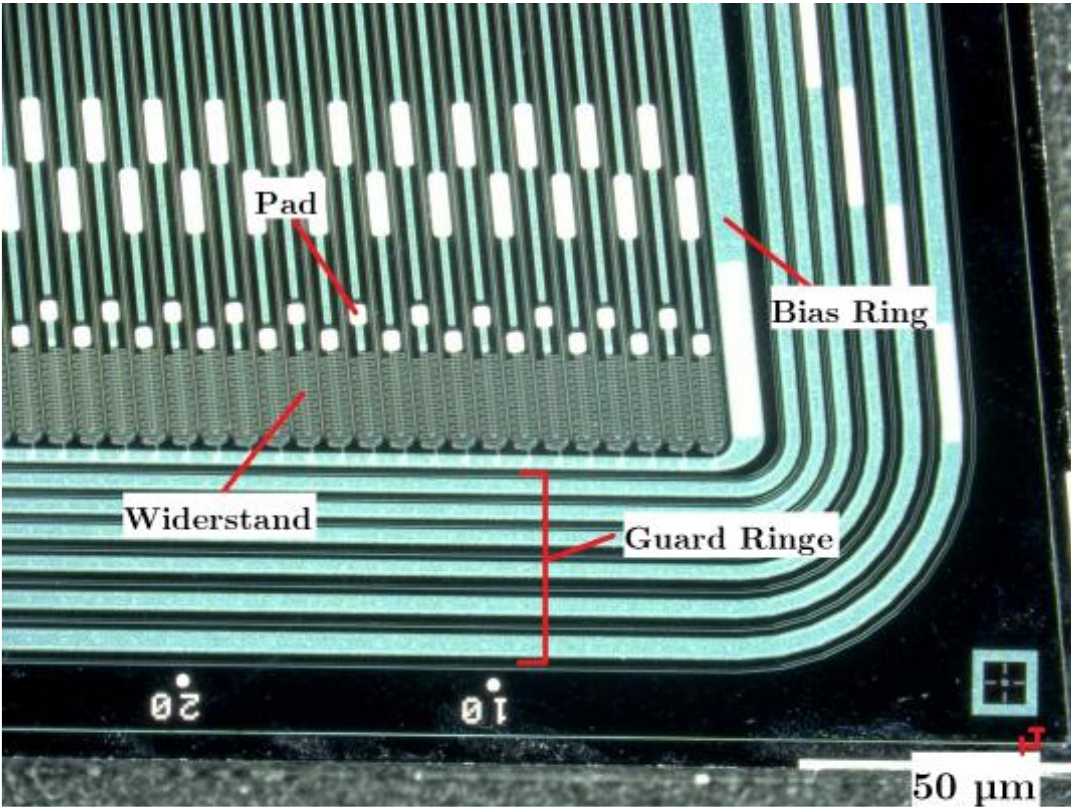
\includegraphics[width=0.5\textwidth]{graphics/Sensor.png}
  \caption{Makroskopische Aufnahmne eines Streifen-Detektors mit entsprechender Kennzeichnung der einzelnen Komponenten \cite{anleitung}.}
  \label{fig:streifendetektor}
\end{figure}
Erhält der Auslesechip ein Signal, weil ein geladenes Teilchen einen Streifen durchquert hat, verstärkt er dieses Signal zunächst und wandelt es in ein Spannungssignal um. Dieses Signal befindet sich dann in einer Pipeline und wird weiter geleitet, wenn ebenfalls ein externes Triggersignal an dem sich hinter dem Streifensensor befindlichen Diodentrigger erhalten wird. Andernfalls werden die Daten verworfen.\\
Um diese Funktionsweise zu erreichen, muss der Silizium-Sensor, wie in Kapitel \ref{sec:Theorie} beschrieben, vollständig depletiert sein. Bei dem im EASy verwendeten Sensor liegt $U_\text{Dep}$ bei ungefähr \SI{60}{\volt} bis \SI{80}{\volt}. Um zu ermitteln, inwiefern der Sensor depletiert ist, wird die Effizienz der Ladunssammlung (\textit{engl.: Charge Collection Effiency} CCE) bestimmt. Maximal ist diese Effizienz, wenn eine vollkommene Depletierung ($U \ge U_\text{Dep}$) vorhanden ist. In diesem Fall lässt sich der Sensor zur Teilchendetektion verwenden. Die CCE kann durch
\begin{equation}
  \text{CCE}(U) = \frac{1 - \exp\left(\frac{-d_\text{c}(U)}{a}\right)}{1 - \exp\left(\frac{-D}{a}\right)}
  \label{eqn:20}
\end{equation}
bestimmt werden. Diese Formel gilt jedoch nur für Photonen, daher wird diese Messung mit dem eingebauten Laser durchgeführt. Hierbei ist $d_\text{c}$ die Dicke der Depletionszone, $D$ die Sensordicke und $a$ die Eindringtiefe des Lasers in das Silizium.

\FloatBarrier
\subsection{Lasereinheit}
\label{sec:Lasereinheit}
Die Abbildung \ref{fig:Gehäuse} stellt das äußere Gehäuse des Detektors dar und es lässt sich erkennen, dass auf diesem vertikal zum Sensor ein Reiter sitzt. In diesem ist der für die Untersuchung der Detektoreigenschaften notwendige Laser.
\begin{figure}[htb]
  \centering
  \includegraphics[width=0.9\textwidth]{graphics/Gehäuse.png}
  \caption{Fotographie des EASy Gehäuses mit integriertem Laser und Carbon-Plätchen,
  sowie den einzelnen Anschlüssen \cite{anleitung}.}
  \label{fig:Gehäuse}
\end{figure}
Dieser kann in Laser(L)- oder in Quell(Q)-Position
gestellt werden, je nachdem, welche Messung durchgeführt werden soll.
Die emittiert Wellenlänge des Lasers beträgt \SI{980}{\nano\meter}
mit einem minimalen Durchmesser von \SI{20}{\micro\meter}, einer Pulslänge von
\SI{5}{\nano\second} und einer Leistung von \SI{0.6}{\milli\watt}.
An dem Reiter sind zwei Miktrometerschrauben angebracht, um die Position des Lasers in der Horizontalen verschieben zu können und in der Vertikalen zu fokusieren.

\FloatBarrier
\subsection{Kontrolleinheit}
Mit der in Abbildung \ref{fig:control} dargestellten Kontrolleinheit wird der Detektor gesteuert. Dabei wird mit einem Flachbandkabel eine Verbindung zwischen Detektoreinheit und Kontrolleinheit
hergestellt. Der entsprechende Anschluss befindet sich auf dem Sockel mit der Aufschrift \textit{Sensor Unit}. An dieser Stelle können zudem für die Lasermessungen ein Glasfaserkabel und für die Quellmessungen ein Triggerkabel angeschlossen werden. Der Drehknopf \textit{Diode Bias} ermöglicht das Einstellen einer bestimmte Vorspannung auf den Bias Ring, die dieser an die Streifen überträgt. Diese wird zusammen mit dem auftretenden Strom im Kontrollfenster angezeigt. Die Stromversorgung der Kontrolleinheit befindet sich auf der Rückseite des Gerätes.
\begin{figure}[htb]
  \centering
  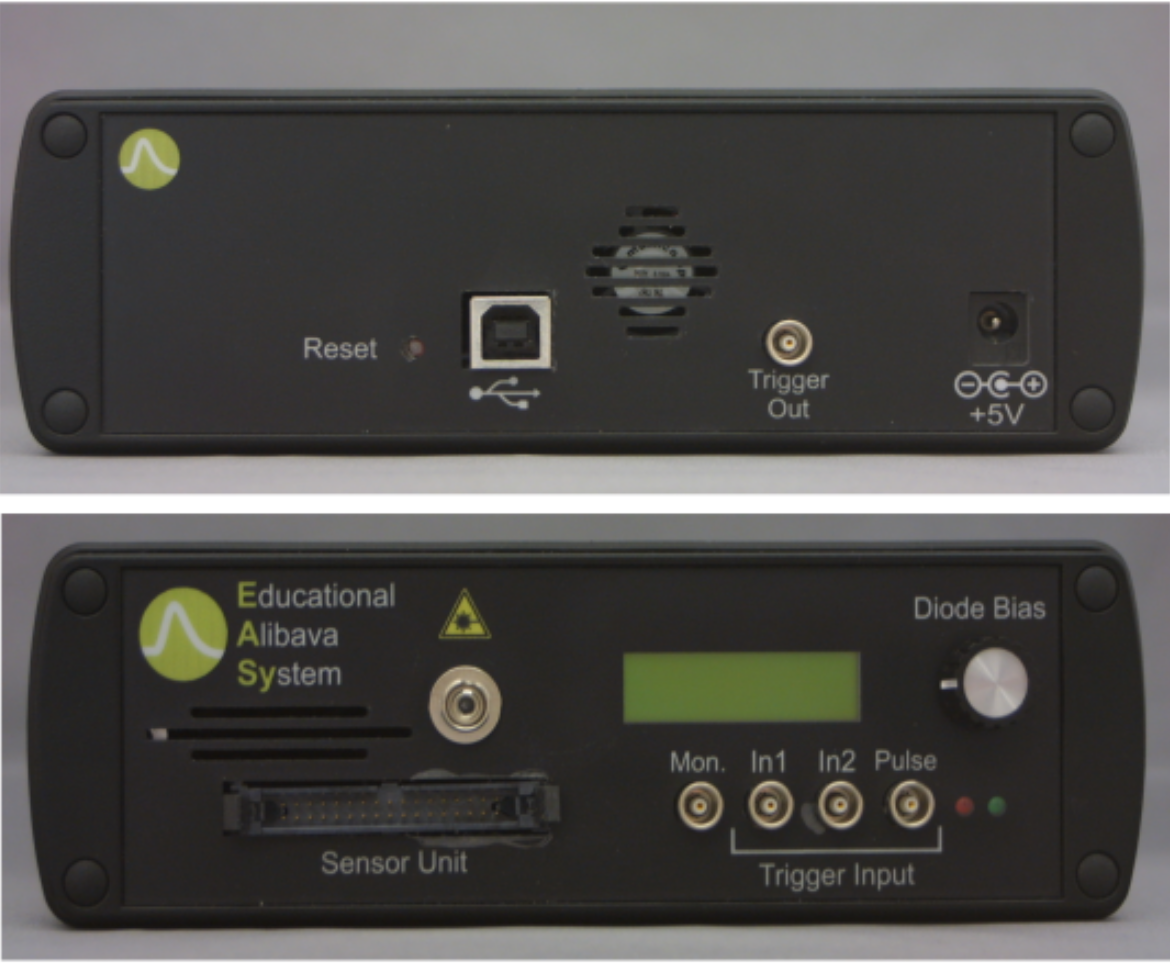
\includegraphics[width=0.4\textwidth]{graphics/Control.png}
  \caption{Front- und Rückansicht der Kontrolleinheit und ihrer Anschlüsse \cite{anleitung}.}
  \label{fig:control}
\end{figure}
Die Abbildung \ref{fig:aufbau} zeigt eine schematische Darstellung des gesamten Versuchsaufbau.
\begin{figure}[htb]
  \centering
  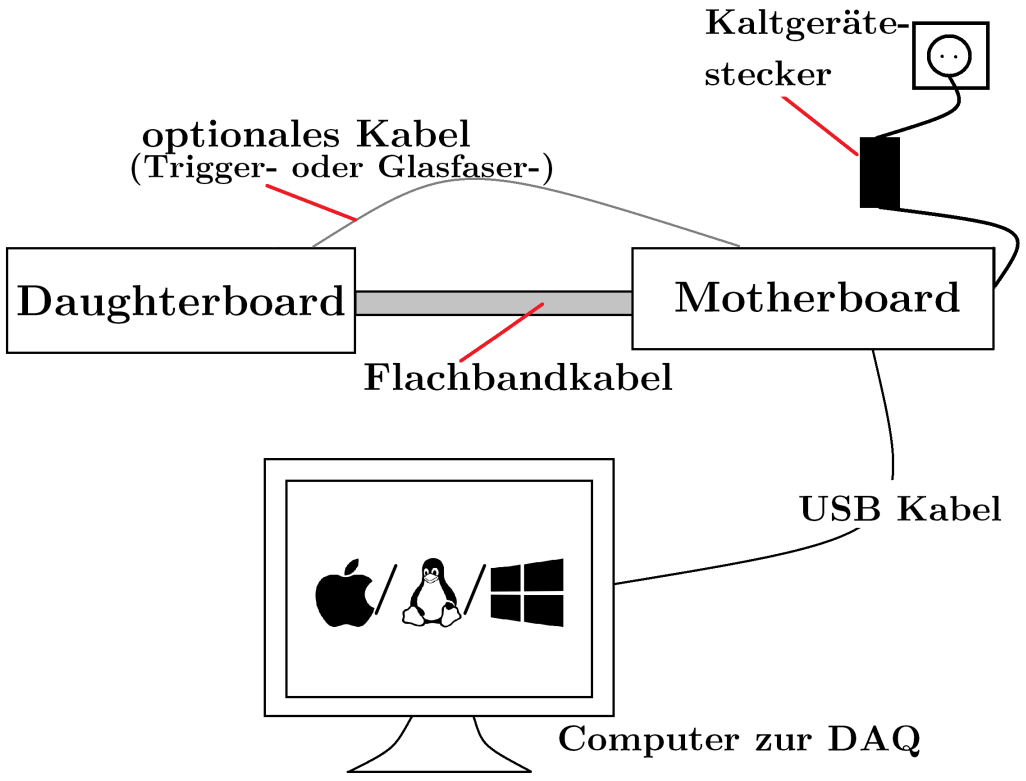
\includegraphics[width=0.5\textwidth]{graphics/Aufbau.png}
  \caption{Graphischer Aufbau des kompletten Versuches mit Detektoreinheit
  (Daughterboasrd), Kontrolleinheit (Motherboard) und Computer \cite{anleitung}.}
  \label{fig:aufbau}
\end{figure}
Aus strahlenschutztechnischen Gründen befindet sich die Detektoreinheit für die Messung mit der Sr-Quelle in einer Kiste mit einer Bleiabschirmung, damit keine radioaktive Strahlung nach außen gelangen kann. Dies ist in Abbildung \ref{fig:quell} erkennbar.
\begin{figure}[htb]
  \centering
  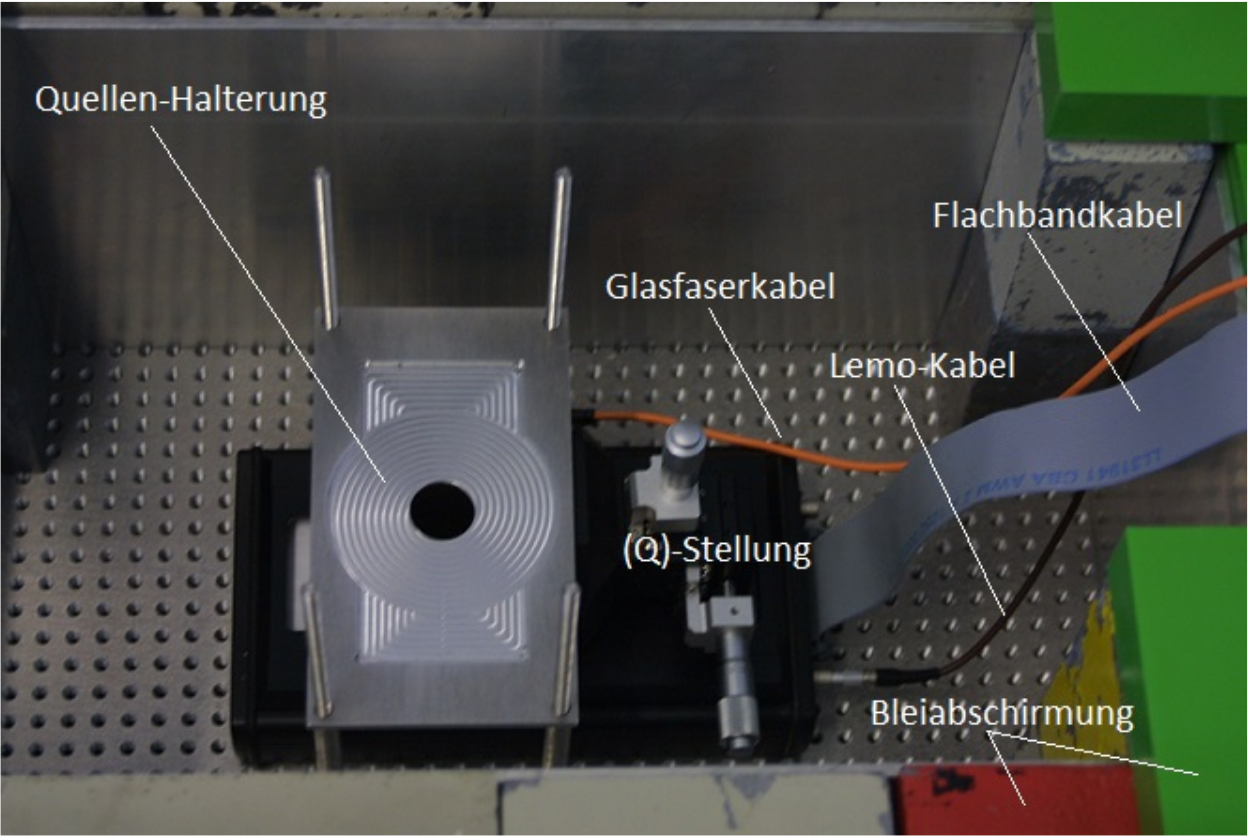
\includegraphics{graphics/Abschirmung.png}
  \caption{Vertikale Sicht auf die Detektoreinheit in horizontaler Bleiabschirmung \cite{anleitung}.}
  \label{fig:quell}
\end{figure}

\FloatBarrier
\section{Durchführung}
\label{sec:Durchführung}

\subsection{Messung der Strom-Spannungs-Kennlinie}
\label{sec:Kennlinie}
Zur Aufnahme einer Strom-Spannungs-Kennlinie werden zunächste die Detektor- und Kontrolleinheit mit dem Computer verbunden und das zur Steuerung von EASy mitgeführte Programm \textit{Alibava\_gui} gestartet. Zur konkreten Messung muss anschließend die Vorspannung von \SI{0}{\volt} bis einschließlich \SI{200}{\volt} in \SI{10}{\volt} Schritten durchlaufen und der Leckstrom aufgezeichnet werden.\\
Aus dem erhaltenden Verlauf lässt sich die Depletionsspannung abschätzen. Diese ist an dem Übergang von einem linearen zu einem sättigenden Verlauf zu erkennen. Um zu gewährleisten, dass der Sensor vollständig depletiert ist, wird eine ca. \SI{20}{\volt} größere Depletionsspannung gewählt als der ermittelte Wert.

\subsection{Pedestals und Noise}
\label{sec:Auswertung_Noise}
Um Informationen über die Pedestals und Noise zu erhalten, wird eine LogData Pedestal.h5 in einem Ordner Pedestal angelegt und ein \textit{Pedastal Run} mit dem \textit{Alibava\_gui} durchgeführt. Hierbei wird die Messung für 1000 Events durchgeführt.

\subsection{Kalibrationsmessung}
\label{sec:Kalibrationsmessung}
Die Elektronenpulse werden mit Hilfe des Triggersystems in ein digitales Signal umgewandet, welches anschließend über das Flachbandkabel an den Auslesechip gegeben wird um die ADC-Counts in Ladung umzurechnen. Um eine Kalibrationskurve aufzunehmen, wird die Option \textit{Calibration Run} gewählt und im entsprechenden Optionsfenster die Default-Werte der Delay Einstellung wie in Abbildung \ref{fig:calibration-durchfuehrung} angezeigt verwendet. Zunächst wird der Delay-Scan durchgeführt, um eine optimale Verzögerung zwischen eingehenden Signal und Chipauslese zu erhalten. Aus der entstandenen Verteilung lässt sich anschließend ein Maximum bestimmen und der entsprechende Wert wird unter \textit{Settings} und \textit{DAQ} eintragen.\\
\begin{figure}[htb]
  \centering
  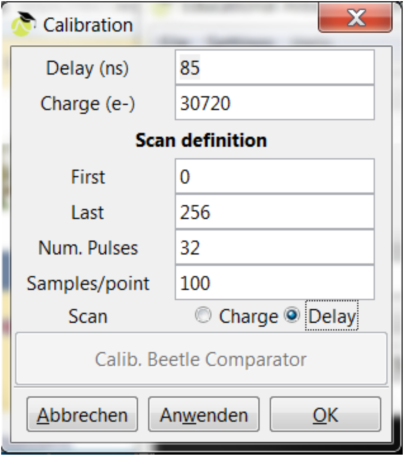
\includegraphics[width=0.3\textwidth]{graphics/Calibration.pdf}
  \caption{Default-Einstellungen der Messung einer Kalibrationskurve zur Bestimmung
  der besten Verzögerung zwischen gebenen Elektronenpuls und Chipauslese \cite{anleitung}.}
  \label{fig:calibration-durchfuehrung}
\end{figure}

Im zweiten Schritt werden fünf verschiedene Kanäle des Auslesechips bzw. Streifen des Streifendetektors ausgewählt und unter \textit{Option} im \textit{Calibration}-Menü nacheinander eingestellt. Für jeden Streifen wird ein Run durchgeführt und die Graphik gespeichert. Für einen der fünf Streifen wird zudem ein Run bei $U=\SI{0}{\volt}$ durchgeführt.

\FloatBarrier
\subsection{Vermessung der Streifendetektoren mittels Laser}
\label{sec:Vermessung_Laser}
Die Streifenstruktur des Sensors lässt sich mit Hilfe eines Lasers untersuchen, da sich oberhalb der Streifen eine Metallisierung befindet, welche das vom Laser emittierte Licht reflektiert und daher den Halbleiter nicht durchdringt.\\
Zu Beginn wird dazu die optimale Verzögerung zwischen Lasersignal und Chipauslese bestimmt. Dafür wird unter \textit{Option} \textit{Laser Sync.} ausgewählt und der Run durchgeführt. Aus dem Maximum der angezeigten Abhängigkeit zwischen gemessenen ADC-Counts und Verzögerung kann nun die optimale Verzögerung abgelesen und unter dem Formularfeld bei \textit{Laser Run} eingetragen werden.\\
Als nächstes wird mit der horizontalen Mikrometerschraube der Peak maximiert. Trifft der Laser möglichst senkrecht auf die Metallisierung, wird der größte Teil reflektiert, sodass nur noch wenig Energie in den Sensor eindringt. Befindet sich der Laser somit genau zwischen zwei Metallisierungen ist der Peak maximal. Von diesem Startpunkt aus wird in \num{35} \SI{10}{\micro\meter}-Schritten ein Laserscan durchgeführt und diese einzelnd gespeichert.


\subsection{Bestimmung der Charge Collection Eficiency}
\label{sec:CCE}
\subsubsection{Unter Verwendung eines Lasers}
Wie im Schritt zuvor wird zu Beginn dieser Messung erst der maximale Peak mit optimaler Verzögerung gesucht. Nun wird allerdings für je \num{1000} Ereignisse (\textit{engl. events}) die Spannung von \SI{0}{\volt} bis \SI{200}{\volt} in \SI{10}{\volt}-Schritten erhöht und ein Run durchgeführt.

\subsubsection{Unter Verwendung einer Sr-Quelle}
Nach der Umplatzierung der Detektoreinheit in den strahlengeschützen Aufbau wird der Laser in die horizontale Ausrichtung gebracht und die Sr-Quelle in Position gebracht. Analog zu der CCE-Bestimmung duch einen Laser wird die Spanung in \SI{10}{\volt}-Schritten von \SI{0}{\volt} bis \SI{200}{\volt} erhöht. Hier werden pro Run der Datensatz auf \num{10000} Events erhöht.

\subsection{Großer Quellscan}
\label{sec:Quellscan}
Für die letzte Messung wird die Spannung wie in der Messung der Strom-Spannungs-Kennlinie auf einen Wert leicht über der Depletionsspannung gesetzt und ein \textit{RS Run} mit einer Anzahl der Events von \num{1000000} durchgeführt und abgespeichert.\\

Durch ein mitgeführtes Programm werden alle \textit{.h5}-Dateien in passende .txt-Dateien
umgewandelt, damit diese für die Auswertung herangezogen werden können.
